Chương này trình bày thiết kế phần cứng của node cảm biến và điều khiển. Nội dung được xây dựng dựa trên sơ đồ nguyên lý của mạch node, trong đó các khối chức năng chính gồm khối nguồn, khối vi điều khiển, khối giao tiếp, khối cảm biến và khối actuator. Việc tách hệ thống thành các khối giúp quá trình thiết kế, kiểm thử và sửa lỗi trở nên rõ ràng hơn, đồng thời làm cơ sở để mở rộng node trong các phiên bản sau.

\section{Yêu cầu thiết kế phần cứng}
Node được thiết kế để hoạt động trong môi trường căn hộ, đặt gần cây trồng hoặc khu vực cần giám sát chất lượng không khí. Do đó phần cứng cần đáp ứng đồng thời các yêu cầu về đo lường, truyền thông và điều khiển thiết bị. Node phải đọc được dữ liệu từ nhiều cảm biến khác nhau, truyền dữ liệu về gateway qua LoRa, nhận lệnh điều khiển từ gateway và điều khiển các cơ cấu chấp hành như relay hoặc bộ phát hồng ngoại.

Các yêu cầu chính của phần cứng gồm:
\begin{itemize}
    \item Cung cấp được các mức nguồn cần thiết cho vi điều khiển, cảm biến, LoRa và relay.
    \item Có khả năng đọc cảm biến analog như TDS, pH và ánh sáng.
    \item Có khả năng giao tiếp với cảm biến digital thông qua I2C, UART hoặc GPIO.
    \item Có kênh giao tiếp LoRa để truyền dữ liệu không dây về gateway ESP32.
    \item Có mạch relay để đóng cắt quạt, đèn hoặc thiết bị ngoài.
    \item Có mạch phát hồng ngoại để điều khiển điều hòa.
    \item Có đầu nối mở rộng để thuận tiện đấu dây cảm biến và kiểm thử.
\end{itemize}

Vì node sử dụng Arduino Pro Mini nên tài nguyên xử lý, số chân vào ra và bộ nhớ đều có giới hạn. Điều này ảnh hưởng trực tiếp đến cách bố trí chân, định dạng gói tin và thuật toán xử lý trên node. Thiết kế phần cứng cần ưu tiên sự ổn định và dễ kiểm tra hơn là tích hợp quá nhiều chức năng phức tạp vào một node duy nhất.

\begin{figure}[h!]
    \centering
    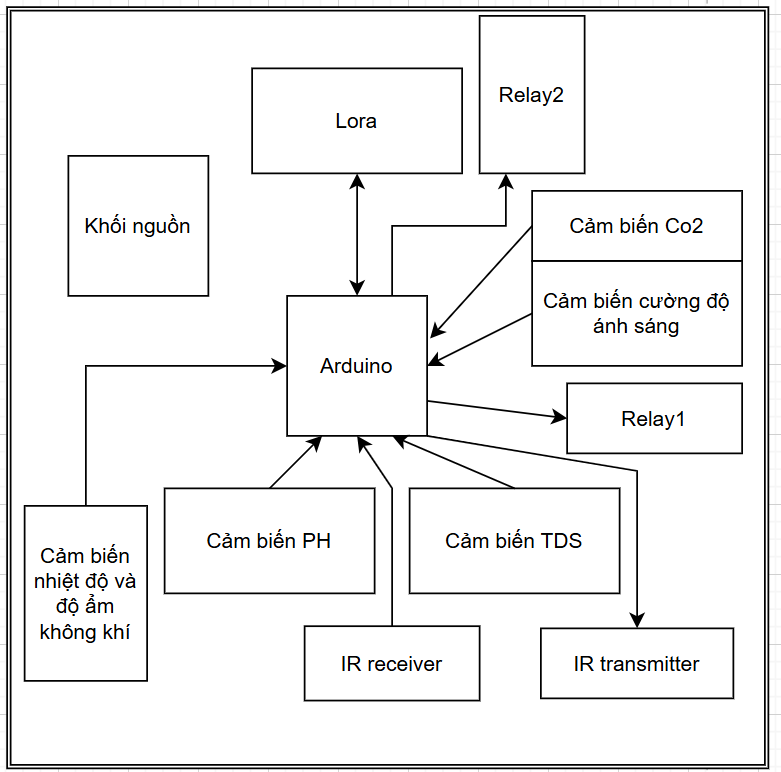
\includegraphics[width=\textwidth]{chapter4/image/node.png}
    \caption{Kiến trúc phần cứng tổng thể của node}
    \label{fig:node_hardware_overview}
\end{figure}

\section{Phân rã chức năng theo khối}
Từ sơ đồ nguyên lý, node được chia thành năm khối chính. Khối nguồn nhận điện áp đầu vào và tạo ra các mức nguồn ổn định. Khối vi điều khiển sử dụng Arduino Pro Mini làm trung tâm xử lý. Khối giao tiếp gồm LoRa RA-02 và mạch giao tiếp RS485 dự phòng hoặc mở rộng. Khối cảm biến gồm các đầu nối cho cảm biến TDS, pH, ánh sáng, nhiệt độ, độ ẩm và CO2. Khối actuator gồm relay và mạch phát IR.

\begin{longtable}{|p{3.5cm}|p{4.2cm}|p{5.2cm}|}
\hline
\textbf{Khối} & \textbf{Thành phần chính} & \textbf{Vai trò trong hệ thống} \\
\hline
Khối nguồn & Jack DC, diode bảo vệ, module hạ áp, AMS1117-3.3V, tụ lọc, LED báo nguồn & Tạo các mức nguồn 24V, 5V và 3.3V; bảo vệ mạch khỏi đấu ngược cực và giảm nhiễu nguồn. \\
\hline
Khối vi điều khiển & Arduino Pro Mini, các header P1, P2, P4 & Đọc cảm biến, xử lý dữ liệu, điều khiển relay/IR và giao tiếp với LoRa. \\
\hline
Khối giao tiếp & RA-02 LoRa, MAX485, header RS485 & Truyền dữ liệu không dây về gateway và hỗ trợ giao tiếp mở rộng có dây khi cần. \\
\hline
Khối cảm biến & Header TDS, pH, ánh sáng, I2C, analog & Kết nối các cảm biến đo môi trường và điều kiện chăm sóc cây. \\
\hline
Khối actuator & Relay RL1, RL2, RL3; transistor; diode dập xung; LED IR & Bật/tắt quạt, đèn, tải ngoài và phát lệnh hồng ngoại điều khiển điều hòa. \\
\hline
\end{longtable}

Việc phân rã này cũng hỗ trợ quá trình kiểm thử. Khi một chức năng không hoạt động, có thể cô lập lỗi theo từng khối: kiểm tra nguồn trước, sau đó kiểm tra vi điều khiển, đường giao tiếp, cảm biến và cuối cùng là tải điều khiển. Đây là nguyên tắc quan trọng đối với các mạch IoT tự thiết kế vì lỗi có thể xuất phát từ cả phần cứng, dây nối, nhiễu nguồn lẫn chương trình điều khiển.

\section{Nguyên tắc bố trí chân và tín hiệu}
Arduino Pro Mini có số chân hạn chế, trong khi hệ thống cần kết nối nhiều ngoại vi. Do đó các chân được phân nhóm theo chức năng. Nhóm SPI dùng cho LoRa gồm \texttt{MOSI}, \texttt{MISO}, \texttt{SCK}, \texttt{NSS}, \texttt{DIO0} và \texttt{RST}. Nhóm analog dùng cho cảm biến TDS, pH, ánh sáng hoặc cảm biến analog khác. Nhóm digital dùng cho relay, IR LED, tín hiệu điều khiển MAX485 và các cảm biến digital.

Khi thiết kế, các tín hiệu có tốc độ cao hoặc nhạy nhiễu cần được ưu tiên đường đi ngắn và rõ ràng. Tín hiệu SPI đến LoRa nên tránh chạy gần đường cấp relay hoặc tải công suất. Các đường analog từ cảm biến pH và TDS cần hạn chế nhiễu vì tín hiệu đo thường nhỏ và dễ bị ảnh hưởng bởi nguồn, relay hoặc dây dài.

\begin{longtable}{|p{3.2cm}|p{4cm}|p{5.8cm}|}
\hline
\textbf{Nhóm tín hiệu} & \textbf{Tín hiệu đại diện} & \textbf{Ghi chú thiết kế} \\
\hline
SPI LoRa & \texttt{MOSI}, \texttt{MISO}, \texttt{SCK}, \texttt{NSS} & Dùng cho module RA-02, yêu cầu mức logic phù hợp với 3.3V. \\
\hline
Điều khiển LoRa & \texttt{RST}, \texttt{DIO0} & Dùng reset module và nhận ngắt khi có gói tin. \\
\hline
Analog cảm biến & \texttt{Po}, \texttt{A}, \texttt{OUT} & Đọc pH, ánh sáng, TDS hoặc cảm biến analog tương tự. \\
\hline
Actuator & \texttt{RL1}, \texttt{RL2}, \texttt{RL3}, \texttt{TX} & Điều khiển relay và LED hồng ngoại. \\
\hline
I2C & \texttt{SCL}, \texttt{SDA} & Kết nối cảm biến nhiệt độ, độ ẩm hoặc module mở rộng. \\
\hline
UART/RS485 & \texttt{UITXo}, \texttt{UIRXo}, \texttt{UIENo} & Kết nối MAX485 hoặc cảm biến công nghiệp nếu mở rộng. \\
\hline
\end{longtable}

Trong thiết kế thực tế, việc đặt tên net rõ ràng giúp giảm nhầm lẫn khi lập trình. Các tên như \texttt{RL1}, \texttt{RL2}, \texttt{Po}, \texttt{TDS}, \texttt{DIO0}, \texttt{NSS} tạo liên hệ trực tiếp giữa sơ đồ nguyên lý và mã nguồn firmware. Đây là điểm quan trọng vì phần mềm và phần cứng của hệ thống được phát triển song song.
